\subsection{Autenticação \emph{Digest} HTTP}

A autenticação \emph{Digest}, proposta na RFC 2019 \cite{RFC2019} e definida como padrão na RFC 
2617, foi desenvolvida para ser uma alternativa mais compatível e segura para a autenticação básica, 
corrigindo as falhas mais graves da mesma, como a falta de criptografia de senhas, vulnerabilidade a 
captura e repetição de pacotes e proteção contra vários outros tipos comuns de ataques 
\cite{GOURLEY2002}.

Assim como a autenticação básica HTTP, a \emph{Digest} é baseada no paradigma 
desafio-resposta \cite{RFC7616}. A diferença está na adição de diversos parâmetros nos 
cabeçalhos, utilizados para identificação única de desafios, nível de qualidade de proteção, 
especificação de algoritmo de \emph{hashing} utilizado dentre outros \cite{CHAPMAN2012}. Por padrão, 
o algoritmo utilizado é o MD5, porém na RFC 7616 foram adicionados e recomendados os algoritmos 
SHA-256 e SHA-512/256 \cite{RFC7616}.

O parâmetro \texttt{response} é a principal parte do cabeçalho \texttt{Authorization}: ele contém 
uma concatenação criptografada de dados da requisição, como nome do usuário, \texttt{realm}, senha, 
método HTTP, URL (\emph{Uniform Resource Locator}), entre outros parâmetros, todos separados por dois pontos \cite{CHAPMAN2012}. O 
cliente realiza o cálculo resultante no valor de \texttt{response}, assim como o servidor, que 
compara o valor calculado com o valor recebido. Caso as credenciais sejam válidas, o servidor retorna
o status HTTP 200 (OK) e o cabeçalho \texttt{Authentication-Info}, que contém parâmetros utilizados 
para uma futura autenticação, autenticação mútua e reenvio de parâmetros para confirmação de 
legitimidade (Figura \ref{fig:digestAuth}).

\begin{figure}[ht]
  \centering
  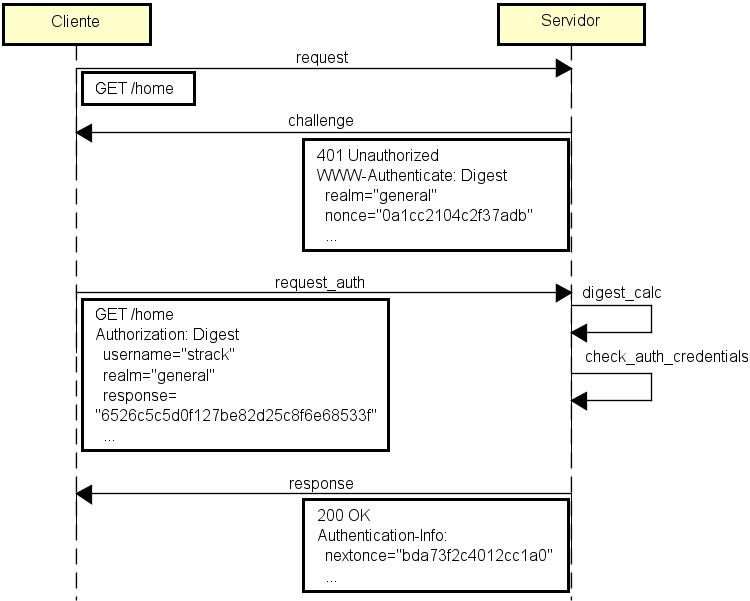
\includegraphics[width=.9\textwidth]{Digest Authentication (Simplified).png}
  \caption{Exemplo de autenticação \emph{Digest}.}
  \label{fig:digestAuth}
\end{figure}